\section{Circle Class Reference}
\label{classCircle}\index{Circle@{Circle}}
Inheritance diagram for Circle::\begin{figure}[H]
\begin{center}
\leavevmode
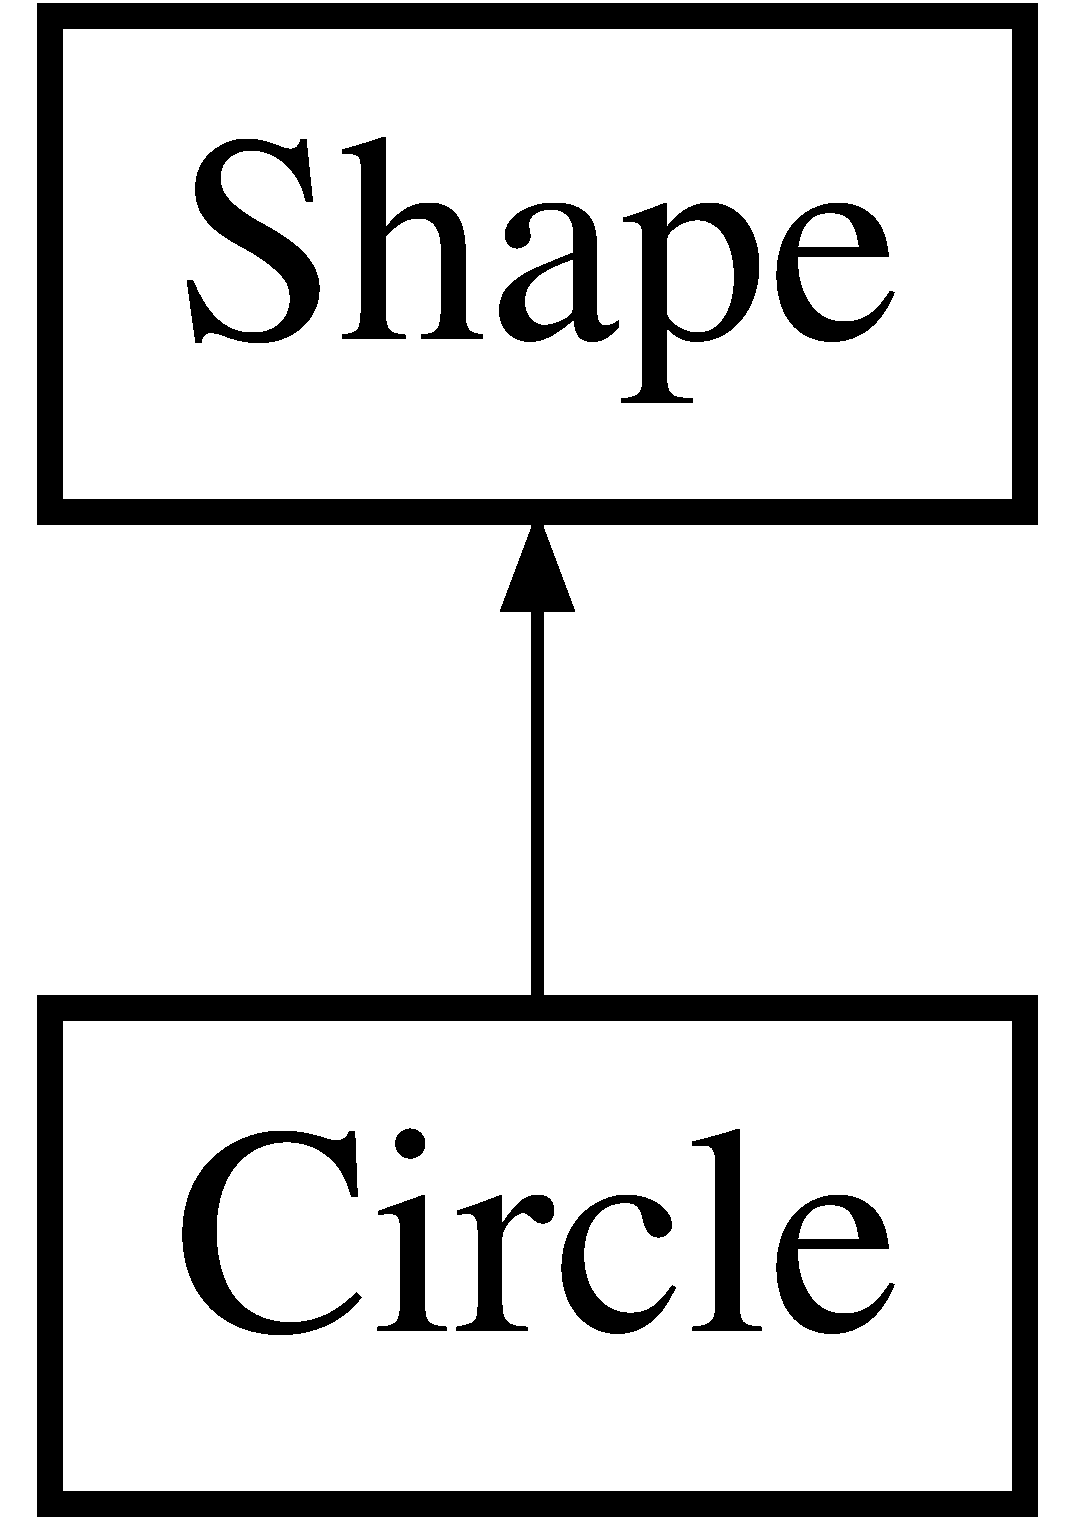
\includegraphics[height=2cm]{classCircle}
\end{center}
\end{figure}
\subsection*{Public Member Functions}
\begin{CompactItemize}
\item 
{\bf Circle} (double radius)\label{classCircle_05c707753451188c26b43508b610ff8e}

\item 
Number {\bf get\-Area} ()\label{classCircle_31746d74f86226e3c35561a3f0cccf9b}

\end{CompactItemize}
\subsection*{Package Attributes}
\begin{CompactItemize}
\item 
Double {\bf area}\label{classCircle_a8d702f9c81180ccaabd7277e156b56c}

\end{CompactItemize}


\subsection{Detailed Description}




Definition at line 22 of file Test\-Return\-Inheritance.java.

The documentation for this class was generated from the following file:\begin{CompactItemize}
\item 
Test\-Return\-Inheritance.java\end{CompactItemize}
